\documentclass[11pt,a4paper]{article}
\usepackage[margin=1in]{geometry}
\usepackage[T1]{fontenc}
\usepackage[utf8]{inputenc}
\usepackage{lmodern}
\usepackage{hyperref}
\usepackage{enumitem}
\usepackage{xurl}
\usepackage{tikz}
\usepackage{float}
\usetikzlibrary{arrows.meta, positioning, shapes.geometric}
\hypersetup{colorlinks=true,linkcolor=blue,urlcolor=blue}
\newcommand{\codepath}[1]{\path{#1}}
\tikzset{box/.style={rectangle,draw,rounded corners,align=center,inner sep=3pt,minimum width=36mm},decision/.style={diamond,draw,aspect=2.1,align=center,inner sep=2pt},line/.style={-Latex}}

\title{Phase-1 Deliverable: CI Hooks}
\author{SIT Engine Architecture}
\date{\today}

\begin{document}
\maketitle

\section{Technical Description}
CI Hooks provide automated regression gates so semantic drift is detected before merge. They connect validation scripts to PR/push lifecycle events.

For Phase-1 completion criteria, these hooks are the enforcement layer for parity against the Phase-0 Tenstorrent Wormhole baseline behavior.

\section{Implementation Fulfillment}
Implemented in \codepath{.github/workflows/phase1-ci.yml}. Workflow triggers on \texttt{push} and \texttt{pull\_request}, sets up Python, installs dependencies, and runs \texttt{python tests/run\_golden\_suite.py --outdir /tmp/golden\_out\_ci}. Any non-zero exit fails the job and blocks merge.

\subsection*{Phase-0 Baseline Provenance (Verified)}
\begin{itemize}[leftmargin=*]
  \item Source repo: \url{git@github.com:Srinidhi-Magesh08/Tenstorrent_test_raw_files.git}
  \item Baseline branch/commit: \texttt{main} @ \texttt{4512ce4e1a689f64c866160bf1f8e7e5e3e2ec89}
  \item Baseline run artifact: \codepath{phase0_golden/tt_run_2026-02-09/raw_profiler/profile_log_device.csv}
  \item Run header baseline: \texttt{ARCH=wormhole\_b0}, \texttt{CHIP\_FREQ[MHz]=1000}, \texttt{Max Compute Cores=64}
\end{itemize}

\section{Design \& Architecture}
CI remains orchestration-only: checkout, environment setup, dependency install, semantic validation execution, and fail-fast gating. Validation logic stays in test scripts, preserving separation of concerns.

\subsection*{Function Flowchart}
\begin{figure}[H]
\centering
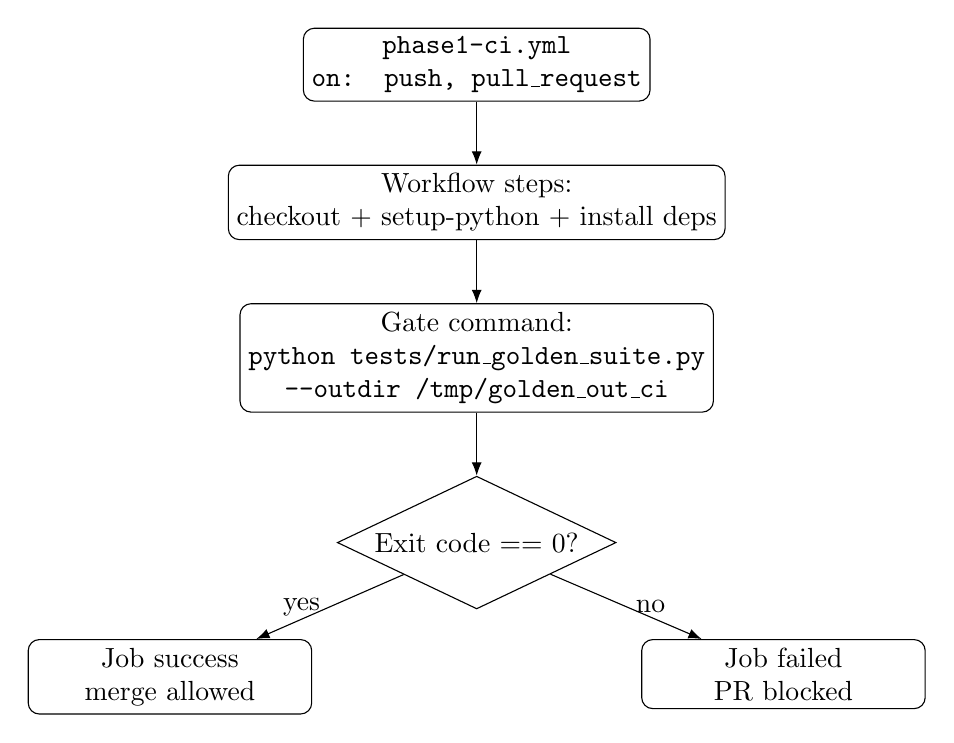
\begin{tikzpicture}[node distance=8mm and 12mm]
\node[box] (a) {\texttt{phase1-ci.yml}\\\texttt{on: push, pull\_request}};
\node[box, below=of a] (b) {Workflow steps:\\checkout + setup-python + install deps};
\node[box, below=of b] (c) {Gate command:\\\texttt{python tests/run\_golden\_suite.py}\\\texttt{--outdir /tmp/golden\_out\_ci}};
\node[decision, below=of c] (d) {Exit code == 0?};
\node[box, below left=of d] (e1) {Job success\\merge allowed};
\node[box, below right=of d] (e2) {Job failed\\PR blocked};
\draw[line] (a) -- (b);
\draw[line] (b) -- (c);
\draw[line] (c) -- (d);
\draw[line] (d) -- node[left]{yes} (e1);
\draw[line] (d) -- node[right]{no} (e2);
\end{tikzpicture}
\caption{CI Hooks Function Flow}
\end{figure}

\end{document}
